\documentclass[11pt]{article}

\usepackage[margin=1in]{geometry}
\usepackage[T1]{fontenc}
\usepackage{lmodern}
\usepackage{amsmath}
\usepackage{graphicx}
\usepackage{booktabs}
\usepackage{enumitem}
\usepackage{caption}
\usepackage[most]{tcolorbox}
\usepackage[colorlinks=true,linkcolor=blue!50!black,urlcolor=blue!50!black]{hyperref}

\graphicspath{{../figures/}{./}}
\captionsetup{font=small,labelfont=bf}
\setlist{itemsep=2pt}
\setlength{\parskip}{4pt}

% A "plain words" box for the key idea of each section
\newtcolorbox{idea}{colback=blue!4,colframe=blue!45!black,boxrule=0.6pt,arc=2pt,
  left=6pt,right=6pt,top=4pt,bottom=4pt,fonttitle=\bfseries,title=In one sentence}
% An interview question and answer
\newtcolorbox{qa}[1]{colback=black!3,colframe=black!35,boxrule=0.5pt,arc=2pt,
  left=6pt,right=6pt,top=3pt,bottom=3pt,fonttitle=\bfseries\color{black},
  coltitle=black,colbacktitle=black!8,title={Q: #1}}

\title{The Switchable Barrier Project, Explained in Plain English}
% TODO: replace with your full name
\author{Aditya M.}
\date{A companion guide to the technical report \\[2pt]
\small\url{https://github.com/adityameenak/switchable-barrier-runaway}}

\begin{document}
\maketitle

\noindent This guide explains what the project does, how the computer solves it, how
we know the answers are right, and what was found, without assuming a background in
numerical methods. Each section opens with a one-sentence summary. The last section
lists questions an interviewer is likely to ask, with short answers.

\tableofcontents

% =====================================================================
\section{The problem}

\begin{idea}
When one battery cell overheats, it can set off its neighbours like dominoes, and the
barrier between cells has to both let heat out on normal days and block it on the
worst day.
\end{idea}

A lithium-ion cell stores a lot of chemical energy. If it gets hot enough, roughly
150\,$^\circ$C in this model, chemical reactions inside it start releasing heat. That heat
raises the temperature, which makes the reactions go faster, which releases more heat.
This feedback loop is called \textbf{thermal runaway}, and it ends with the cell at
several hundred degrees.

The danger is what happens next. The hot cell heats its neighbour past 150\,$^\circ$C, the
neighbour runs away too, and so on down the pack. This is called
\textbf{propagation}.

Battery packs put a thin barrier between cells. The barrier has two jobs that pull in
opposite directions:

\begin{center}
\begin{tabular}{@{}lll@{}}
\toprule
 & \textbf{Normal day} (cells gently warm) & \textbf{Worst day} (one cell at 900\,$^\circ$C) \\
\midrule
\textbf{Conductor}  & Good: heat reaches the cooling  & Bad: passes the fire's heat on \\
\textbf{Insulator}  & Bad: traps heat, cells age      & Good: blocks the heat \\
\textbf{Switchable} & Good: acts as a conductor       & Good: acts as an insulator \\
\bottomrule
\end{tabular}
\end{center}

A \textbf{switchable barrier} conducts heat while it is cool and insulates once it gets
hot, like a fuse for heat. The project asks whether that really gives you both
benefits, and what the barrier needs to achieve to do so.

% =====================================================================
\section{What is being simulated}

\begin{idea}
A slice through five cells and four barriers, where the computer tracks how heat moves,
how much heat each cell's chemistry releases, and how the barrier changes as it warms.
\end{idea}

Picture cutting straight through the stack: five cells, each 10\,mm thick, with a 2\,mm
barrier between each pair, and cooling at both ends. The model follows temperature along
that one line, which is why it is called a \textbf{one-dimensional} (1D) model.

\subsection*{The heat equation}

Everything rests on one equation, the heat equation:
\[
  \underbrace{\rho c_p \frac{\partial T}{\partial t}}_{\text{how fast a spot warms}}
  = \underbrace{\frac{\partial}{\partial x}\!\left(k\,\frac{\partial T}{\partial x}\right)}_{\text{heat flowing in minus out}}
  + \underbrace{q}_{\text{heat released there}}
\]
In words: \emph{how fast a spot warms up equals the heat flowing in from its neighbours,
minus the heat flowing out, plus any heat the chemistry releases right there.}

The symbols:
\begin{itemize}
  \item $T$ is temperature, $t$ is time and $x$ is position through the stack.
  \item $\rho c_p$ is how much energy it takes to warm a piece of material by one degree.
  \item $k$ is the \textbf{thermal conductivity}: how easily heat flows through a material.
        The conductor barrier has $k = 5$, the aerogel insulator $k = 0.03$ (in W/m$\cdot$K).
\end{itemize}

\subsection*{The chemistry}

Each piece of a cell carries a number $\alpha$ (alpha) between 0 and 1 that says how far
its reaction has gone: 0 means fresh, 1 means fully burnt. The reaction speed follows the
\textbf{Arrhenius law}, which makes it grow \emph{exponentially} with temperature. That
is the runaway feedback loop written as a formula. A fully reacted cell releases enough
heat to warm itself by 600\,$^\circ$C.

\subsection*{The switch}

The switchable barrier's conductivity depends on its own temperature: 5 below 120\,$^\circ$C
and 0.05 above it, a 100-fold drop, with a smooth transition about 5\,$^\circ$C wide. It
switches back when it cools.

\subsection*{The two tests}

\begin{enumerate}
  \item \textbf{Normal day:} every cell produces a little heat (as when charging). The
        model runs until temperatures stop changing and reports the hottest cell.
  \item \textbf{Worst day:} cell 1 starts at 300\,$^\circ$C and everything else at
        25\,$^\circ$C. Does the runaway spread?
\end{enumerate}

\noindent One honest caveat: every material number is an order-of-magnitude placeholder,
not a measurement of a real cell. The trends are the result; the exact numbers are not
predictions.

% =====================================================================
\section{How the computer solves it}

\begin{idea}
The stack is cut into small slabs, heat is passed between neighbouring slabs like money
between bank accounts, and each time step does the chemistry and the heat flow
separately, using methods that cannot blow up.
\end{idea}

\subsection*{Cutting the stack into slabs (finite volumes)}

A computer cannot handle a continuous line, so the stack is chopped into small slabs:
40 per cell and 12 per barrier. The program keeps one temperature per slab and works out
how much heat crosses each boundary between neighbouring slabs. This is the
\textbf{finite-volume method}.

Its big advantage is bookkeeping. Heat leaving one slab is exactly the heat entering the
next, like a transfer between two bank accounts, so the method never creates or destroys
energy by accident.

\subsection*{The boundary between two materials (harmonic mean)}

Where a cell meets an aerogel barrier, the conductivity jumps by a factor of 27. The
program needs one conductivity for the boundary between those two slabs. A simple
average would be badly wrong, because heat flow is limited by the \emph{worst}
conductor, just as water through two pipes in a row is limited by the narrow one. The
correct answer is to add the two \emph{resistances} in series, which gives the
\textbf{harmonic mean}. It is exact for layered materials.

\subsection*{One step at a time, two processes (operator splitting)}

Each time step is done in two moves:

\begin{enumerate}
  \item \textbf{Chemistry first,} holding temperature fixed for a moment. The reaction
        equation then has an \emph{exact} solution:
        \[
          \alpha_\text{new} = 1 - (1-\alpha_\text{old})\,e^{-\text{rate}\times\Delta t}.
        \]
        This matters because the reaction can be astronomically fast. A naive update
        (``rate times time step'') would overshoot and blow up. The exponential form can
        never push $\alpha$ past 1, however big the step, and it adds exactly the
        matching amount of heat, so energy still balances.
  \item \textbf{Heat flow second,} using \textbf{backward Euler}, an \emph{implicit}
        method. ``Implicit'' means it solves for all the future temperatures at once
        instead of extrapolating from the current ones. That keeps it stable at any step
        size. Because each slab only talks to its two neighbours, the equations form a
        simple pattern (a \emph{tridiagonal} system) that a computer solves almost
        instantly.
\end{enumerate}

\subsection*{Small steps only when needed (adaptive time stepping)}

While a cell is igniting, the program takes tiny steps (no slab may heat by more than
2\,$^\circ$C from chemistry in one step). When nothing dramatic is happening it takes steps
of up to half a second. This keeps the run accurate without being slow: each simulation
takes under a second.

% =====================================================================
\section{How we know it is right}

\begin{idea}
Eighteen automatic tests compare the code against answers we already know, and they run
on GitHub every time the code changes.
\end{idea}

Anyone can write code that produces nice-looking plots. Tests are what make a simulation
believable:

\begin{enumerate}
  \item \textbf{Energy conservation.} Seal both ends so no heat can escape, and turn the
        chemistry off. Total energy should never change. It stays constant to 12 decimal
        places.
  \item \textbf{A known exact answer.} Steady heat flow through cell, barrier, cell has a
        textbook solution (resistances in series). The code matches it to within
        $10^{-8}$\,$^\circ$C.
  \item \textbf{One reacting slab with no losses.} It must end exactly 600\,$^\circ$C hotter,
        and its ignition time must match a high-accuracy professional solver within 1\%.
  \item \textbf{Convergence.} Make the slabs smaller or the time steps shorter, and the
        answer should settle down to a fixed value. If it keeps changing, the simulation is
        measuring the grid rather than the physics.
\end{enumerate}

% =====================================================================
\section{Three things the work uncovered}

\begin{idea}
The convergence test exposed a real flaw in the textbook chemistry, and two smaller
surprises changed how the switch and the cooling were modelled.
\end{idea}

\subsection*{(a) The reaction was too fast for any grid}

At first, refining the grid kept changing the answer. The time for the fire to reach
cell 2 went 14.3\,s, 10.9\,s, 11.1\,s, 8.8\,s as the slabs got smaller, with no sign of
settling.

The reason: the reaction constants describe how a cell \emph{starts} to fail, between
about 150 and 250\,$^\circ$C. Using the same formula for a burning cell at 900\,$^\circ$C gives
a reaction rate of around a billion per second. A reaction that fast would happen in a
zone about 0.1 micrometres thick, thousands of times thinner than a slab, so no practical
grid could resolve it.

Real chemistry does not keep accelerating forever: at high temperatures, reactions are
limited by how fast the chemicals can reach each other. So the model caps the rate at one
per second. That leaves the start of the reaction unchanged, widens the reaction zone to
about 0.6\,mm, and the answer converges: 20.9, 17.2, 15.9, 15.6, 15.6 seconds
(Figure~\ref{fig:conv}).

\begin{figure}[h]
  \centering
  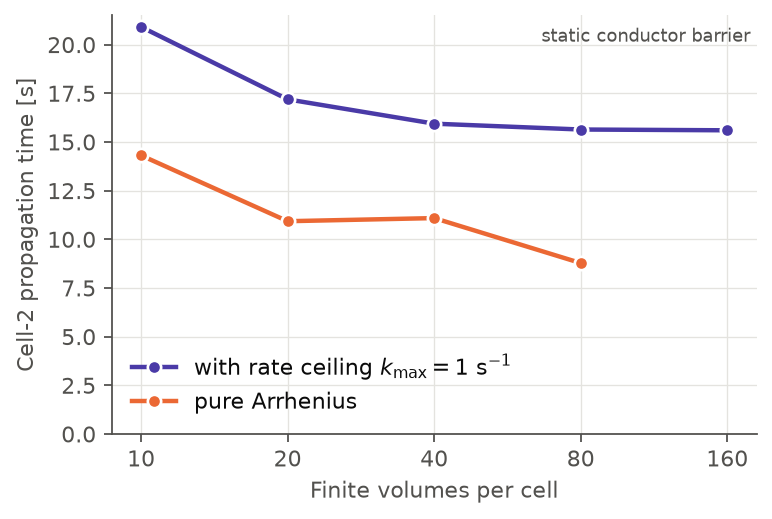
\includegraphics[width=0.6\linewidth]{fig_convergence.png}
  \caption{Time for the fire to reach cell 2 as the grid gets finer. Without the rate cap
  (orange) it never settles; with the cap (purple) it converges.}
  \label{fig:conv}
\end{figure}

\subsection*{(b) The switch needed a log-scale blend}

Blending the conductivity \emph{linearly} between 5 and 0.05 left the barrier three to
four times too conductive until about 20\,$^\circ$C past the switch point, so it barely
switched. Blending the \emph{logarithm} of the conductivity instead makes the transition
behave sensibly at both ends.

\subsection*{(c) In 1D, end cooling decides everything}

With weak cooling at the ends, even a perfect insulator failed to stop the fire. In this
model the ends are the only way for heat to leave. If the burning cell cannot get rid of
its energy through the end, that energy eventually leaks through any barrier. The model
therefore uses strong end cooling (like a plate connected to a cooling system), and this
is listed as a limitation.

% =====================================================================
\section{What we found}

\begin{idea}
The switchable barrier kept cells as cool as a conductor on a normal day and stopped the
fire at the first cell like an insulator, and three simple design rules fall out of the
results.
\end{idea}

\subsection*{The tradeoff}

\begin{center}
\begin{tabular}{@{}lcc@{}}
\toprule
Design & Hottest cell, normal day & Cells that burned \\
\midrule
No barrier       & 37.8\,$^\circ$C & 5 of 5 \\
Conductor        & 38.0\,$^\circ$C & 5 of 5 \\
Insulator        & 64.5\,$^\circ$C & 1 of 5 \\
Switchable       & 38.0\,$^\circ$C & 1 of 5 \\
\bottomrule
\end{tabular}
\end{center}

With no barrier or a conductor, a new cell caught fire about every 15 seconds and the
whole stack was gone in about a minute (Figure~\ref{fig:cells}).

\begin{figure}[h]
  \centering
  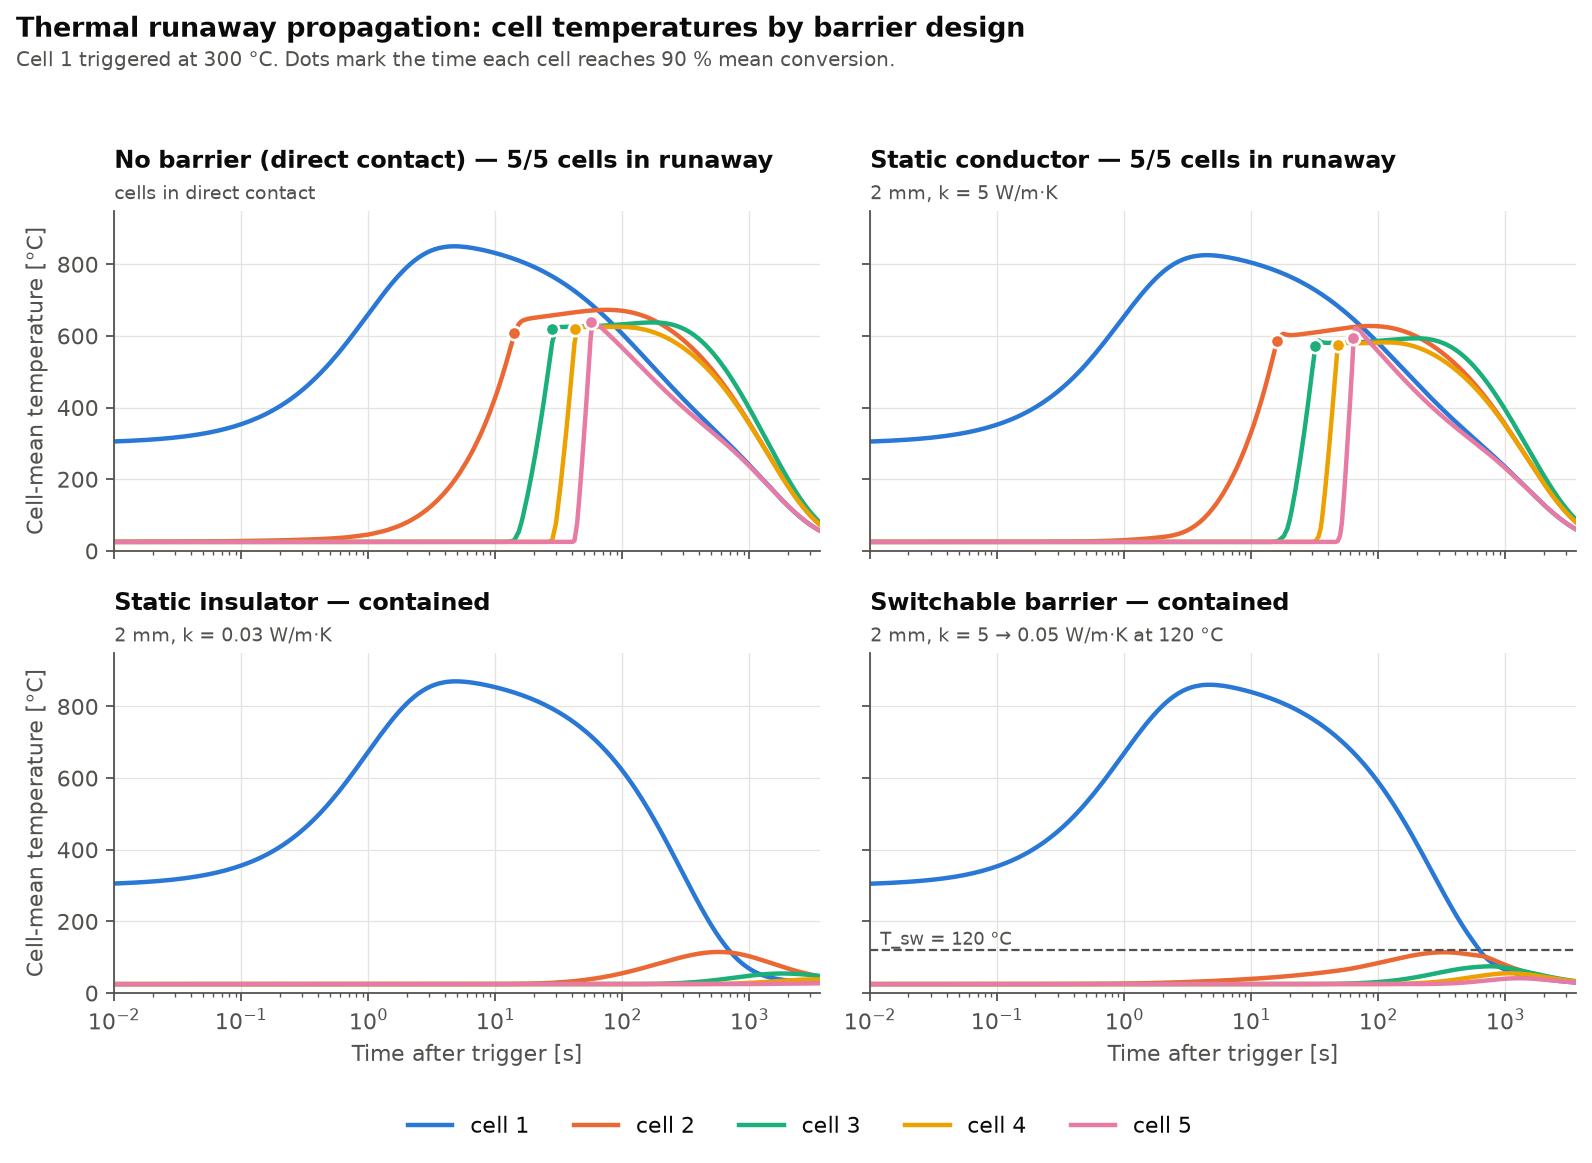
\includegraphics[width=\linewidth]{a_cell_temperatures.png}
  \caption{Average temperature of each cell after cell 1 is triggered, one panel per
  design.}
  \label{fig:cells}
\end{figure}

\subsection*{Why the switch works}

The side of the barrier facing the burning cell heats past 120\,$^\circ$C, switches off,
and holds back a drop of about 700\,$^\circ$C across a couple of millimetres. Meanwhile the
burning cell gets rid of its heat through the cooled end (Figure~\ref{fig:heat}).

\begin{figure}[h]
  \centering
  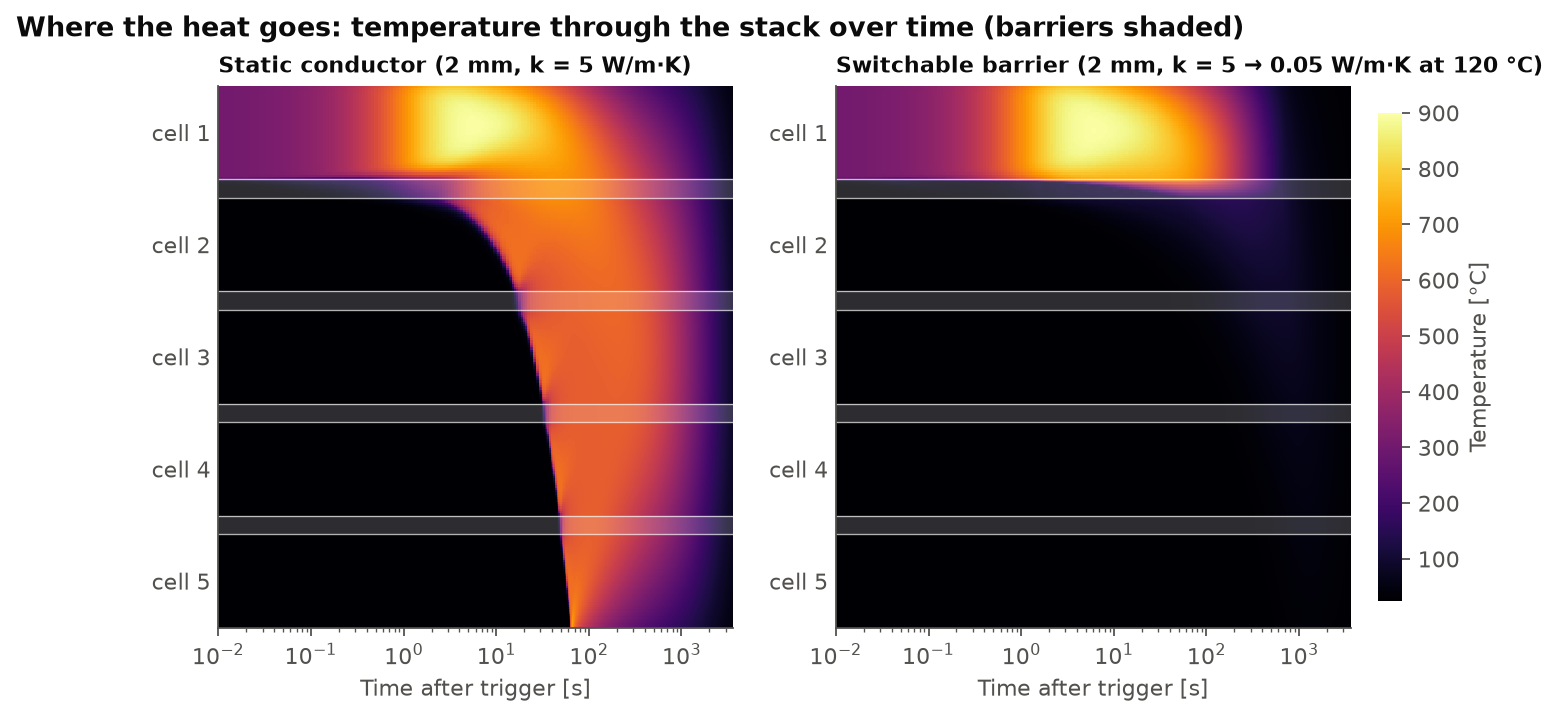
\includegraphics[width=\linewidth]{b_spacetime_heatmap.png}
  \caption{Temperature through the stack over time. Left: the conductor, with a fire
  front sweeping across. Right: the switchable barrier holding the heat in cell 1.}
  \label{fig:heat}
\end{figure}

One subtle point: only the hot side of the switchable barrier insulates. Its cold side
stays below 120\,$^\circ$C and keeps conducting, so the insulating layer is effectively
thinner than the barrier. As a result, cell 2 got hotter behind the switch (153\,$^\circ$C)
than behind the static insulator (124\,$^\circ$C). It still did not ignite, but the margin
is thinner.

\subsection*{Three design rules from 361 simulations}

\begin{enumerate}
  \item \textbf{All or nothing.} Every run ended with either 1 cell burnt or all 5, never
        2 to 4. Once cell 2 ignites it is just as bad a trigger as cell 1, so the barrier
        must win the very first hand-off.
  \item \textbf{One number decides it.} Containment depends on the barrier's hot-state
        conductivity divided by its thickness, which must stay below about
        32\,W/m$^2\cdot$K, roughly a third of the end cooling. The burning cell must lose
        heat to the coolant faster than it leaks it to its neighbour.
  \item \textbf{The switch temperature has a window.} Below about 38\,$^\circ$C the barrier
        switches off on normal days and traps heat. Above about 175\,$^\circ$C it switches
        only after cell 2 has started heating itself, which is too late. Anywhere in
        between works.
\end{enumerate}

\begin{figure}[h]
  \centering
  \begin{minipage}[t]{0.49\linewidth}
    \centering
    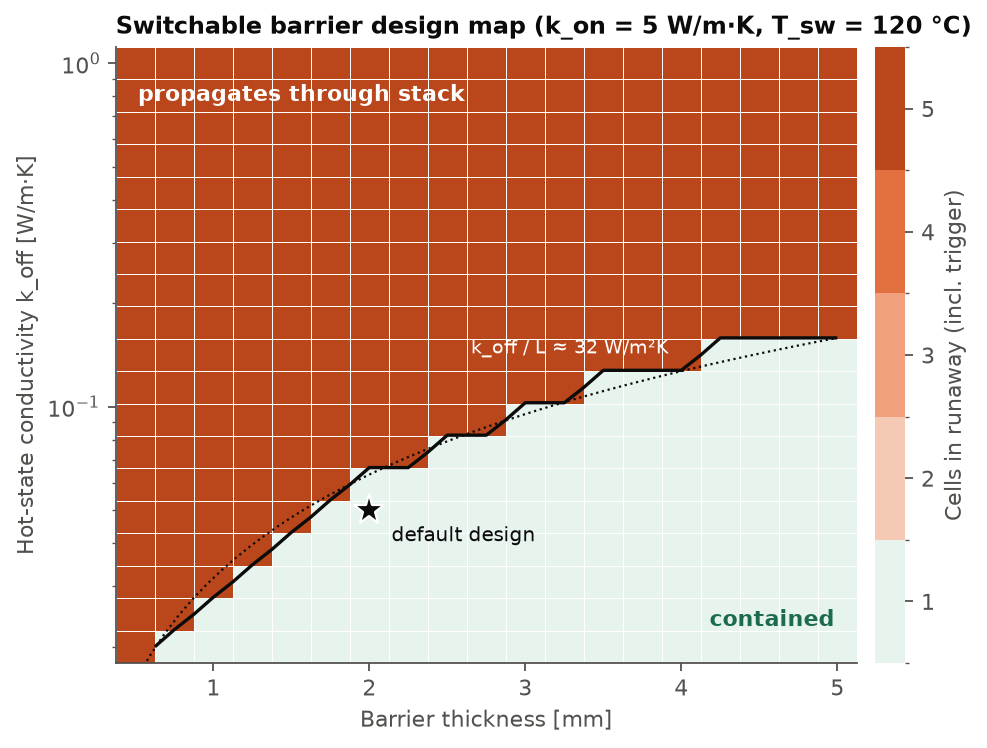
\includegraphics[width=\linewidth]{d_design_map.png}
    \caption{Design map: green is contained, orange means the fire spread to every cell.}
  \end{minipage}\hfill
  \begin{minipage}[t]{0.49\linewidth}
    \centering
    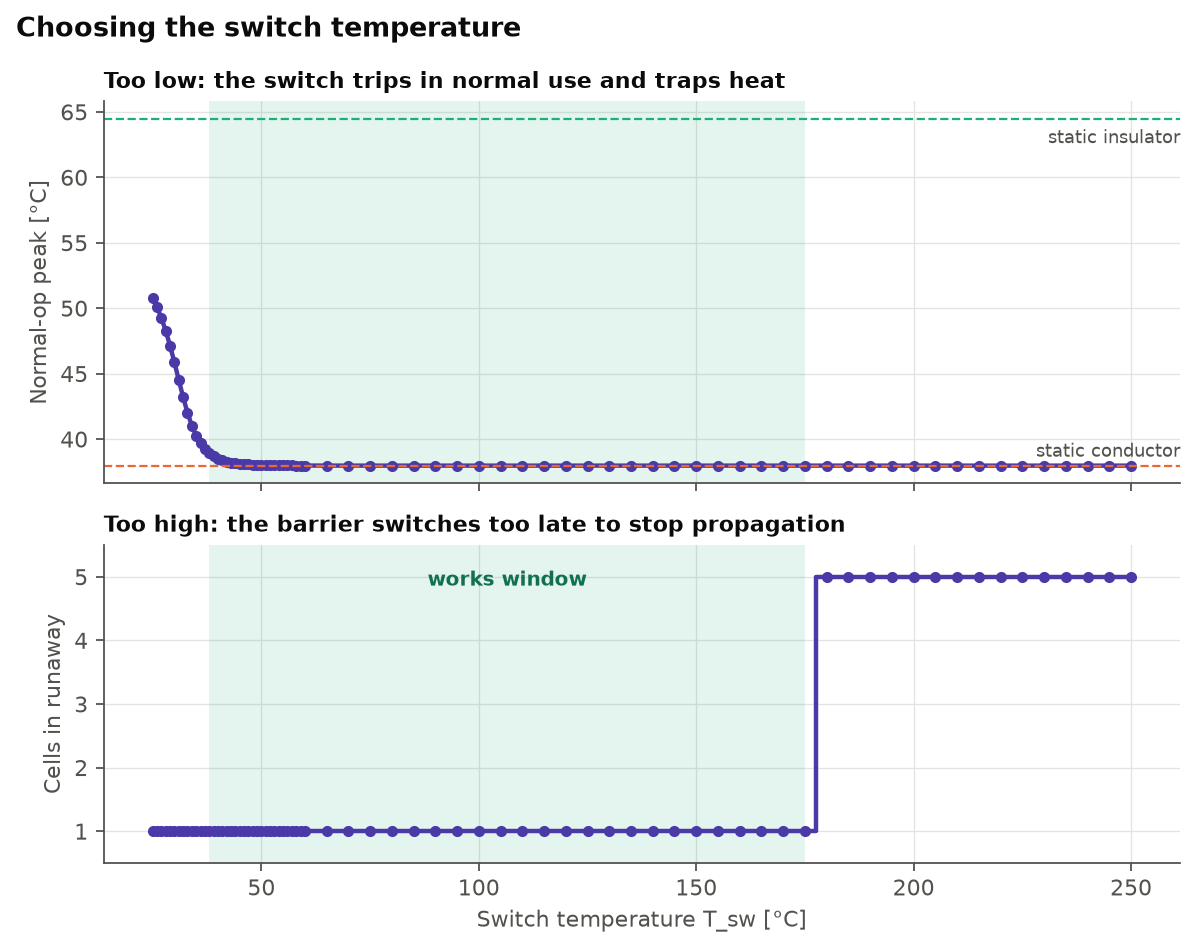
\includegraphics[width=\linewidth]{e_switch_temperature.png}
    \caption{The switch-temperature window where the barrier both cools and protects.}
  \end{minipage}
\end{figure}

% =====================================================================
\section{What this model cannot tell you}

\begin{idea}
It is a deliberately simple model, so its results are trends, not predictions.
\end{idea}

\begin{itemize}
  \item \textbf{One dimension.} Real packs also lose heat sideways, which is why end
        cooling mattered so much here.
  \item \textbf{One lumped reaction.} Real runaway is a sequence of several reactions.
  \item \textbf{No gases or flames.} In real failures, venting gas and ejected material
        often carry much of the heat.
  \item \textbf{An ideal switch.} It flips instantly, reverses perfectly and never wears
        out.
  \item \textbf{Placeholder numbers.} Nothing was fitted to a real cell or material.
\end{itemize}

% =====================================================================
\section{Questions an interviewer might ask}

\begin{qa}{Why use an implicit method for the heat flow?}
With thin slabs, an explicit method would need tiny time steps to stay stable. An
implicit method is stable at any step size, and the tridiagonal system it produces is
very cheap to solve.
\end{qa}

\begin{qa}{Why the harmonic mean at material boundaries?}
It is the exact series resistance between two slab centres. An ordinary average would
let heat leak through the insulator far too easily.
\end{qa}

\begin{qa}{How do you know the answer is not a numerical artifact?}
Convergence testing: refine the grid and the time step and check that the answer settles.
That test is exactly how I found the unresolvable reaction front.
\end{qa}

\begin{qa}{Isn't the rate cap just a fudge factor?}
It is a documented modelling choice. The reaction constants only describe the start of
runaway, and extending them to 900\,$^\circ$C gives unphysical rates. Ideally the cap would
be fitted to the measured duration of a real runaway event.
\end{qa}

\begin{qa}{Why is energy conservation such a strong test?}
Every process in the model only moves energy around or converts chemical energy to heat.
If the totals ever drift, something in the bookkeeping is wrong. Matching to 12 decimal
places rules out most kinds of bug.
\end{qa}

\begin{qa}{What would you do next?}
Fit the switch's conductivity to measured data for a real material, use multi-step
chemistry fitted to calorimetry measurements, move to 2D with side cooling, and compare
against a commercial finite-element model such as COMSOL.
\end{qa}

% =====================================================================
\section*{Glossary}

\begin{description}[leftmargin=1.2em,style=nextline]
  \item[Thermal runaway] A self-accelerating loop where heat speeds up reactions that
        release more heat.
  \item[Propagation] Runaway spreading from one cell to the next.
  \item[Thermal conductivity ($k$)] How easily heat flows through a material.
  \item[Arrhenius law] A rule where reaction speed rises exponentially with temperature.
  \item[Finite-volume method] Splitting space into small slabs and tracking the heat
        exchanged between neighbours.
  \item[Harmonic mean] The averaging rule for things in series, dominated by the smallest
        value.
  \item[Backward Euler (implicit)] A time-stepping method that solves for the future
        state all at once; stable at any step size.
  \item[Operator splitting] Handling two processes (chemistry and heat flow) one after
        the other within each step.
  \item[Convergence] The answer settling down as the grid and time steps are refined.
  \item[Adiabatic] With no heat lost to the surroundings.
\end{description}

\end{document}
